\newpage
\section{Launch Phase}
\subsection{General Analysis}
	\subsubsection{Requirements	 Analysis}
		\begin{itemize}
			\item Functional Requirements ("system shall do 'requirement' ")
			\item Non-functional Requirements ("system shall be 'requirement' ")
			\item Behavioural Requirements ("how the system shall react")
			\item Performance Requirements ("how well does it have to be done")
		\end{itemize}
		% Functional Table
		\begin{table}[h!]
		\begin{tabular} [b] {| c |  p{3cm} | c | p{10cm} |}
			\hline
			\textbf{ID} & \textbf{Requirement} & \textbf{Reference} & \textbf{Description} \\\hline
			F-1 & Communication &  &  \\ \hline
			F-1.1 & Web Server &  & HTTP communication between the hub and the web server; Web-services are going to be use. \\ \hline
			F-1.2 & System &  & System uses Power Line Communication to send and receive data between the modules and the hub. \\ \hline
			F-1.2.1 & Protocol &  & Not Defined yet... \\ \hline
			F-2 & Routing &  &  \\ \hline
			F-2.1 & Storage &  & Energy stored is routed to the consumers. \\ \hline
			F-2.2 & Producers &  & Energy being produced is routed to the storage devices and if full directly routed to the consumers. \\ \hline
		\end{tabular}
		\caption{Functional: System shall do...}
		\end{table}
		
		% Non-Function Table
		\begin{table}[h!]
			\begin{tabular} [b] {| c |  p{3cm} | c | p{10cm} |}
			\hline
			\textbf{ID} & \textbf{Requirement} & \textbf{Reference} & \textbf{Description} \\\hline
			NF-1 & User Interface &  &  \\ \hline
			NF-1.1 & Web Interface &  & User Friendly; Easy to understand so everyone without energy knowledge could use the system. \\ \hline
			NF-1.2 & HW Interface &  & Simple; User Friendly; Only available for the user of the system. \\ \hline
			NF-2 & Electrical &  &  \\ \hline
			NF-2.1 & Voltage &  & The system work in a range 27.5V +-  10\%.\\ \hline
			NF-2.2 & Current &  & Not defined yet... But very important \\ \hline
		\end{tabular}
		\caption{Non-Function: System shall be...}
		\end{table}
		\newpage
		% Behavioural Table
		\begin{table}[h!]
			\begin{tabular} [b] {| c |  p{3cm} | c | p{10cm} |}
			\hline
			\textbf{ID} & \textbf{Requirement} & \textbf{Reference} & \textbf{Description} \\\hline
			B-1 & Status &  &  \\\hline
			B-1.1 & Webpage &  & Warning will be posted in the webpage interface. \\\hline
			B-1.2 & Physical &  & LEDs will show the current status of the connected device Running / Stand By / Warning. \\\hline
			B-1.3 & Report &  & An email will be sent to the defined user when an error occurs. \\\hline
			B-2 & Energy Control &  &  \\\hline
			B-2.1 & Over-production &  & Change devices status to stand by. \\\hline
			B-2.2 & Under-production &  & Use of the energy store in the input/output module and power grid if it have to be a fast charging. \\\hline
			B-2.3 & Normal-production &  & The energy will be routed from the input devices to the output devices. \\\hline
			B-3 & Disaster Avoid &  & Humidity and Temperature sensor will be placed inside the system housing. \\\hline
			B-3.1 & Humidity &  & "When the humidity is high, stop system." \\\hline
			B-3.2 & Temperature &  & "When temperature is high,  stop system." \\\hline
		\end{tabular}
		\caption{Behavioural: How the system shall react...}
		\end{table}
		
		% Perfomance Table
		\begin{table}[h!]
			\begin{tabular} [b] {| c | p{3cm} | c | p{10cm} |}
			\hline
			\textbf{ID} & \textbf{Requirement} & \textbf{Reference} & \textbf{Description} \\ \hline
			P-1 & Hardware &  &  \\ \hline
			P-1.1 & Housing &  & The housing have to be water-proof and with a good heat dissipation. \\ \hline
		\end{tabular}
		\caption{Performance: How well does it have to be done...}
		\end{table}
		\newpage
	\subsubsection{Problem Domain Analysis}
			\paragraph{Block Diagram: Candidates in the system}
			\begin{itemize}
				\item \textbf{Consumers} Units that consumes power (e.g. light, washing machine, electric car)
				\item \textbf{Producers:} Modules that delivers energy to the hub (e.g. Wind-turbine, photovoltaic-cells)
				\item \textbf{Storage:} Modules that both consumes when the system over produces and "produces" (gives energy to the consumers) when needed (e.g. battery, air compressor). 
				\item \textbf{Temperature:} Unit that measures the outdoor temperature. If the temperature is too high or low it might damage the hardware.
				\item \textbf{Humidity:} Unit that measures the humidity where the system is places. If the humidity is too high the hardware might be damaged.
			\end{itemize}
			\paragraph{Block Diagram: Events in the system}
				\begin{itemize}
					\item TemperatureBelowLimit
					\item TemperatureAboveLimit
					\item HumidityAboveLimit
					\item EnergyAboveLimit
					\item EnergyBelowLimit
					\item InitModule
					\item StartModule
					\item StopModule
					\item StandbyModule
					\item CreateModuleLogFile
					\item LoadModuleLogFile
					\item UpdateModuleLogFile
				\end{itemize}
				\textbf{Table with all the above candidates and event combined:}
				\begin{table}[h!]
					\begin{tabular}{| r | c | c | c | c | c |}
					\hline
					~ & Consumers & Producers & Storage & Temp & Humidity \\ \hline
					TempBellowLimit & ~ & ~ & ~ & X & ~ \\ \hline
					TempAboveLimit & ~ & ~ & ~ & X & ~ \\ \hline
					HumidityAboveLimit & ~ & ~ & ~ & ~ & X \\ \hline
					InitModule & X & X & X & ~ & ~ \\ \hline
					StartModule & X & X & X & ~ & ~ \\ \hline
					StopModule & X & X & X & ~ & ~ \\ \hline
					StandbyModule & ~ & X & X & ~ & ~ \\ \hline
					EnergyAboveLimit & ~ & X & ~ & ~ & ~ \\ \hline
					EnergyBelowLimit & ~ & X & ~ & ~ & ~ \\ \hline
					CreateModuleLogFile & ~ & X & X & ~ & ~ \\ \hline
					LoadModuleLogFile & ~ & X & X & ~ & ~ \\ \hline
					UpdateModuleLogFile & ~ & X & X & ~ & ~ \\ \hline
					\end{tabular}
				\end{table}
			\newpage
			\paragraph{State Machine Diagrams}
				\textbf{ }
				\textbf{Description of the different states: }
				\\ After the initialization of all peripherals connected to the hub, the system enters it enters \textit{Run Mode}.
				The system stays in Run Mode until an event happens, e.g. temperature or humidity reaches their limits,
				a new module is connected, a module should be removed, the system is over-/underproducing, the log should be updated ect. 
				\\\textbf{Standby: }If the system overproduces (produces more energy than there is users for), it can standby some of the energy-producing modules.
				\\\textbf{Start: }Whenever a new module is connected it waits for the user to start up the module, either by using a start button on the hub or from the webpage.
				\\\textbf{Stop: }To securely disconnect a module, the user must use the disconnect button (on the module or from web) to make sure all data is saved.
				\\\textbf{Shut down: }If the system finds itself in a critical condition (temperature, humidity, communication problems) it shuts down it's connected modules,
							        tries to save all available data to the log. Then it sends an message (in form of mail) to the user with the problem where after the module
							        powers off itself. 
				\\\textbf{Connect module: }At first the system checks if it has seen exactly that module before, if that is the case it updates variables from the database
									(uptime, production etc.). If the module is new for the system, it creates it in the database and gives it an unique id.
				\\\textbf{Warning: }Is sent if the system tries to send a submodule in standby- , start- or stop mode, but after a while it has not changed (timeout). 
							    After the timeout state, the system returns to run state. The system might also try to restart the device after a while.
			\newpage
			\begin{figure}[h!]		%Remember to put the h!, to not fuck the sections.
				\begin{centering}
					 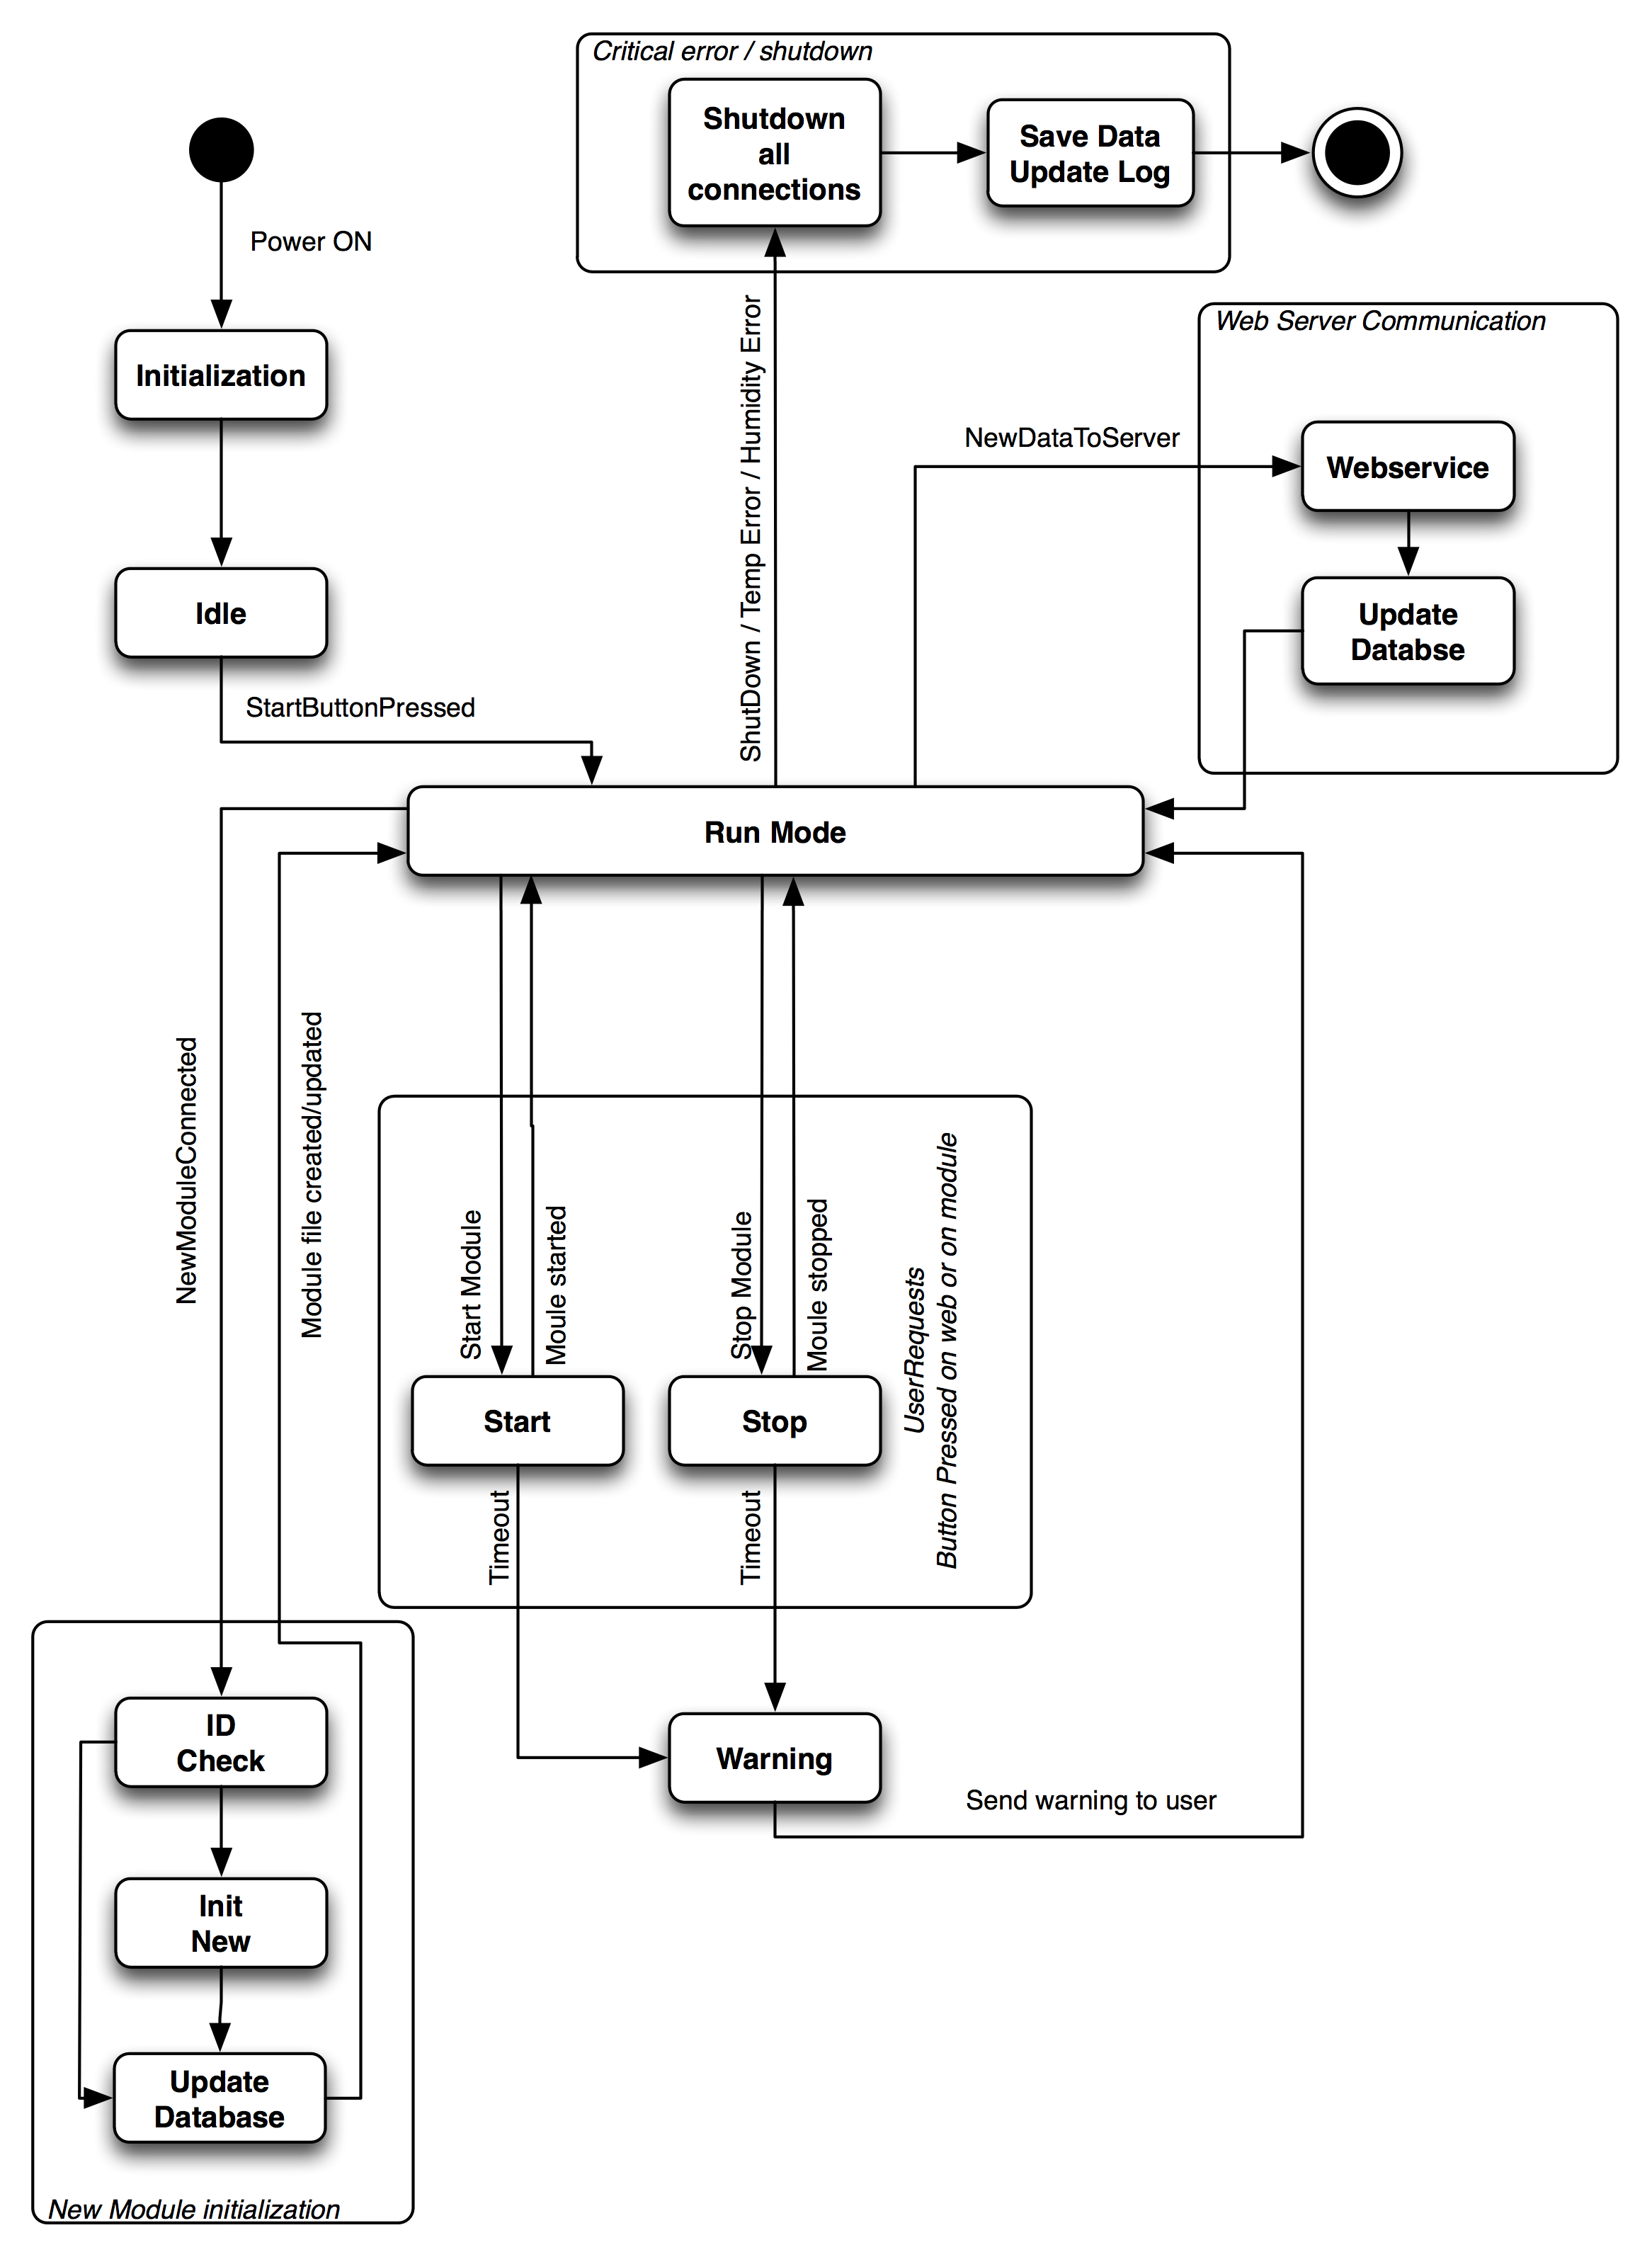
\includegraphics[width=0.8\textwidth]{images/statemachine.png}
		 			\caption{Web user interface}
			 	\end{centering}
			\end{figure}

	\subsubsection{Usage Domain Analysis}
		\textbf{Web user - Log in}
		\\\textit{Description: }
		The log in user is any user with log in to the web interface for the system. This user can manage the energy hub from a browser on a computer.
		\\\textbf{Web user - Visitors}
		\\\textit{Description: }
		This visitor of the web interface can only see info and data in the browser. This user is not able to manage anything.
		\\\textbf{Hub}
		\\\textit{Description: }
		The Hub is the system. the system sometimes have to do something that is not possible for other users.
		\\\textbf{Engineer}
		\\\textit{Description: }
		The engineer is any person with knowledge about how the system works on technical level. This user is able to reprogram the whole system.
		\\\textbf{On system user}
		\\\textit{Description: }
		On system user is any user that go to the physical system and operates on it. This user is able to start and stop parts of the system.
		\\\\\textbf{Plug in module}
		\\\textit{Description: }
		The user should be able to plug in different modules to the system, this is only possible when you stand physical at the system, so this use case is only included for the \textit{On system user}.
		\\\textbf{Unplug module}
		\\\textit{Description: }
		Like plugging in modules this use case is only included for the \textit{On system user}.
		\\\textbf{Start/Stop module}
		\\\textit{Description: }
		The capability of turning modules on and off is included in the \textit{On system user}, \textit{Engineer}, \textit{Hub} and the \textit{Web user - Log in}.
		\\\textbf{Start/Stop system}
		\\\textit{Description: }
		The The capability of turning the system on and off is included in the \textit{On system user}, \textit{Hub} and the \textit{Engineer}. The \textit{Web user - Log in} do not have the option to turn the system on.
		\\\textbf{View Production/Consumption of module}
		\\\textit{Description: }
		It is possible for the \textit{Web user - Log in}, \textit{Web user - Visitors}, \textit{Hub} and the \textit{Engineer}.
		\\\textbf{View temperature}
		\\\textit{Description: }
		It is possible for the \textit{Web user - Log in}, \textit{Web user - Visitors}, \textit{Hub} and the \textit{Engineer}.
		\\\textbf{View log of module}
		\\\textit{Description: }
		It is possible for the \textit{Web user - Log in}, \textit{Hub} and the \textit{Engineer}.
		\\\textbf{View humidity}
		\\\textit{Description: }
		It is possible for the \textit{Web user - Log in}, \textit{Web user - Visitors}, \textit{Hub} and the \textit{Engineer}.
		\\\textbf{Initialize module}
		\\\textit{Description: }
		It is only possible for the \textit{Hub} to initialize modules.
		\\\textbf{Standby a module}
		\\\textit{Description: }
		Setting modules in standby mode is only possible for the \textit{Hub} and the \textit{Engineer}.
		\\\textbf{View energy level of storage modules}
		\\\textit{Description: }
		It is possible for the \textit{Web user - Log in}, \textit{Web user - Visitors}, \textit{Hub} and the \textit{Engineer}.
		\\\textbf{Create log file}
		\\\textit{Description: }
		Creating a log file for a module is only possible for the \textit{Hub}.
		\\\textbf{Disconnect module}
		\\\textit{Description: }
		Disconnecting a module without unplugging it is only possible for the \textit{Hub} and the \textit{Engineer}.
		\\\begin{table}[h!]
					\begin{tabular}{| r | c | c |}
					\hline
					Number	& On system user	& System \\ \hline
					1		& Plug in module	& ~ \\ \hline
					2		& ~					& Initialize module \\ \hline
					3		& Start module		& ~ \\ \hline
					4		& ~					& Turning on the module \\ \hline
					\end{tabular}
				\end{table}
		\\\begin{table}[h!]
					\begin{tabular}{| r | c | c |}
					\hline
					Number	& Hub				& System \\ \hline
					1		& Check the power production (it is to low)	& ~ \\ \hline
					2		& ~											& Setting the module to standby \\ \hline
					\end{tabular}
				\end{table}
	\newpage	
	\subsubsection{Interface Analysis}
	The hardware interface as seen from the users perspective. Note, new modules is connected in the back of the hub.
		\begin{figure}[h!]		%Remember to put the h!, to not fuck the sections.
			\begin{centering}
				 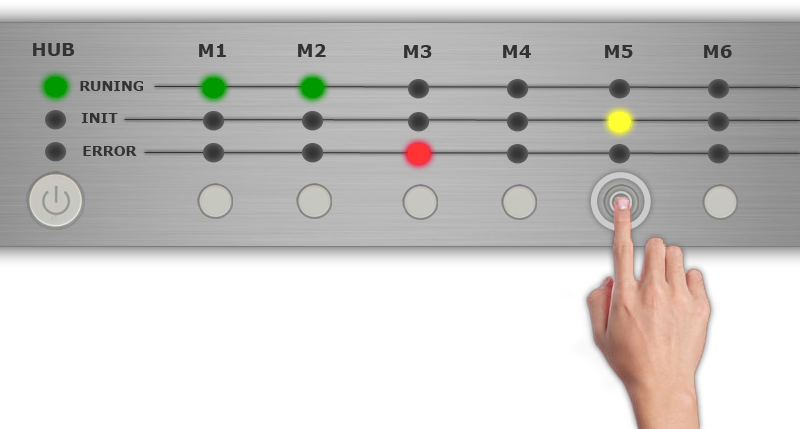
\includegraphics[width=0.8\textwidth]{images/hub_user_interact.png}
				\caption{User interacting with the physical hub module}
		 	\end{centering}
		\end{figure}
		\\ \textbf{The Hub diode states}
		\begin{itemize}
			\item \textbf{Green: }The modules is in Run mode, no problems detected.
			\item \textbf{Yellow: }The module is powered on, but the user has not requested a startup of the module.
							The yellow diode also light up if the user stops the system.
			\item \textbf{Red: }An error has occurred in the system.
		\end{itemize}
		\textbf{Submodules state}
		\begin{itemize}
			\item \textbf{Green: }Constant light, the module is in Run mode, no problems detected. Flashing light, the module is in standby mode, set by the hub
							due to over-/underproduction or other.
			\item \textbf{Yellow: }Constant light, the module is plugged to the hub, but the user has not requested a startup yet or the module has been stopped.
							During initialization (a startup has been requested) the diode flashes.
			\item \textbf{Red: }An error has occurred with the connected module.
		\end{itemize}
		\newpage
		The web-interface. In the little comic book user interaction with the system is shown.
		\begin{figure}[h!]		%Remember to put the h!, to not fuck the sections.
			\begin{centering}
				 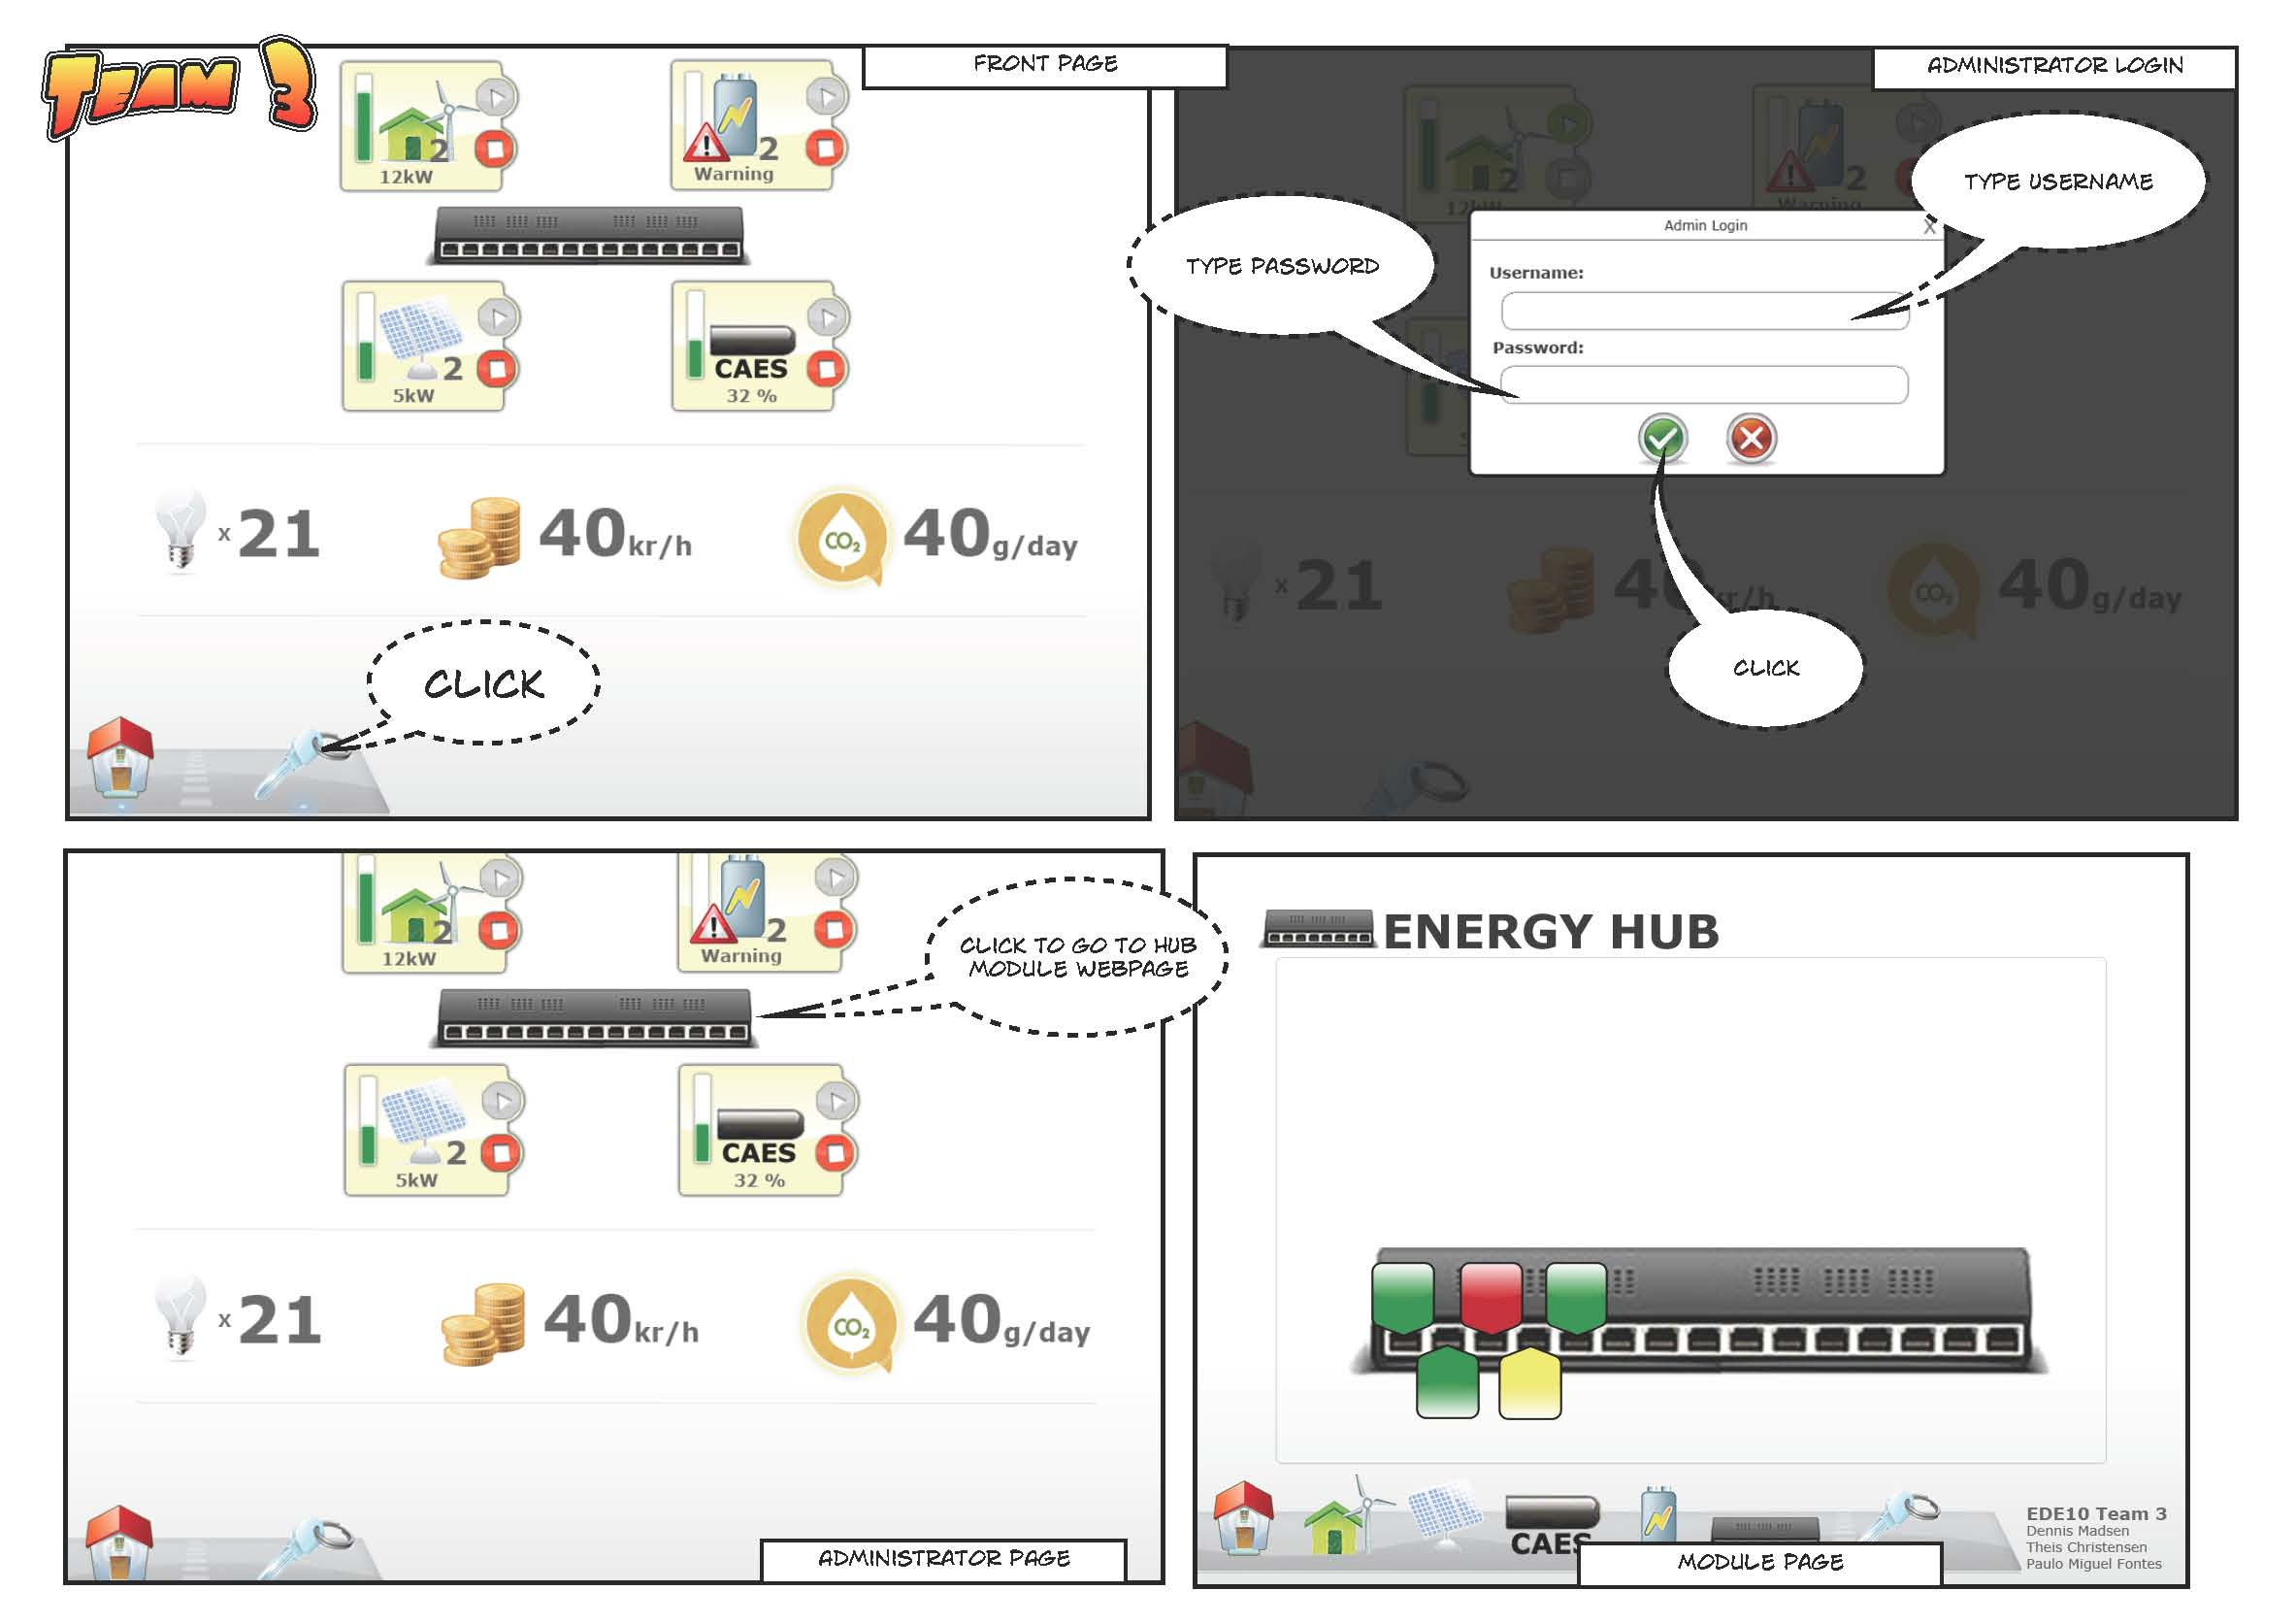
\includegraphics[width=0.82\textwidth]{images/web_interface1.jpg}
				\caption{Web interface; user interaction with the web interface}
		 	\end{centering}
		\end{figure}

		\begin{figure}[h!]		%Remember to put the h!, to not fuck the sections.
			\begin{centering}
				 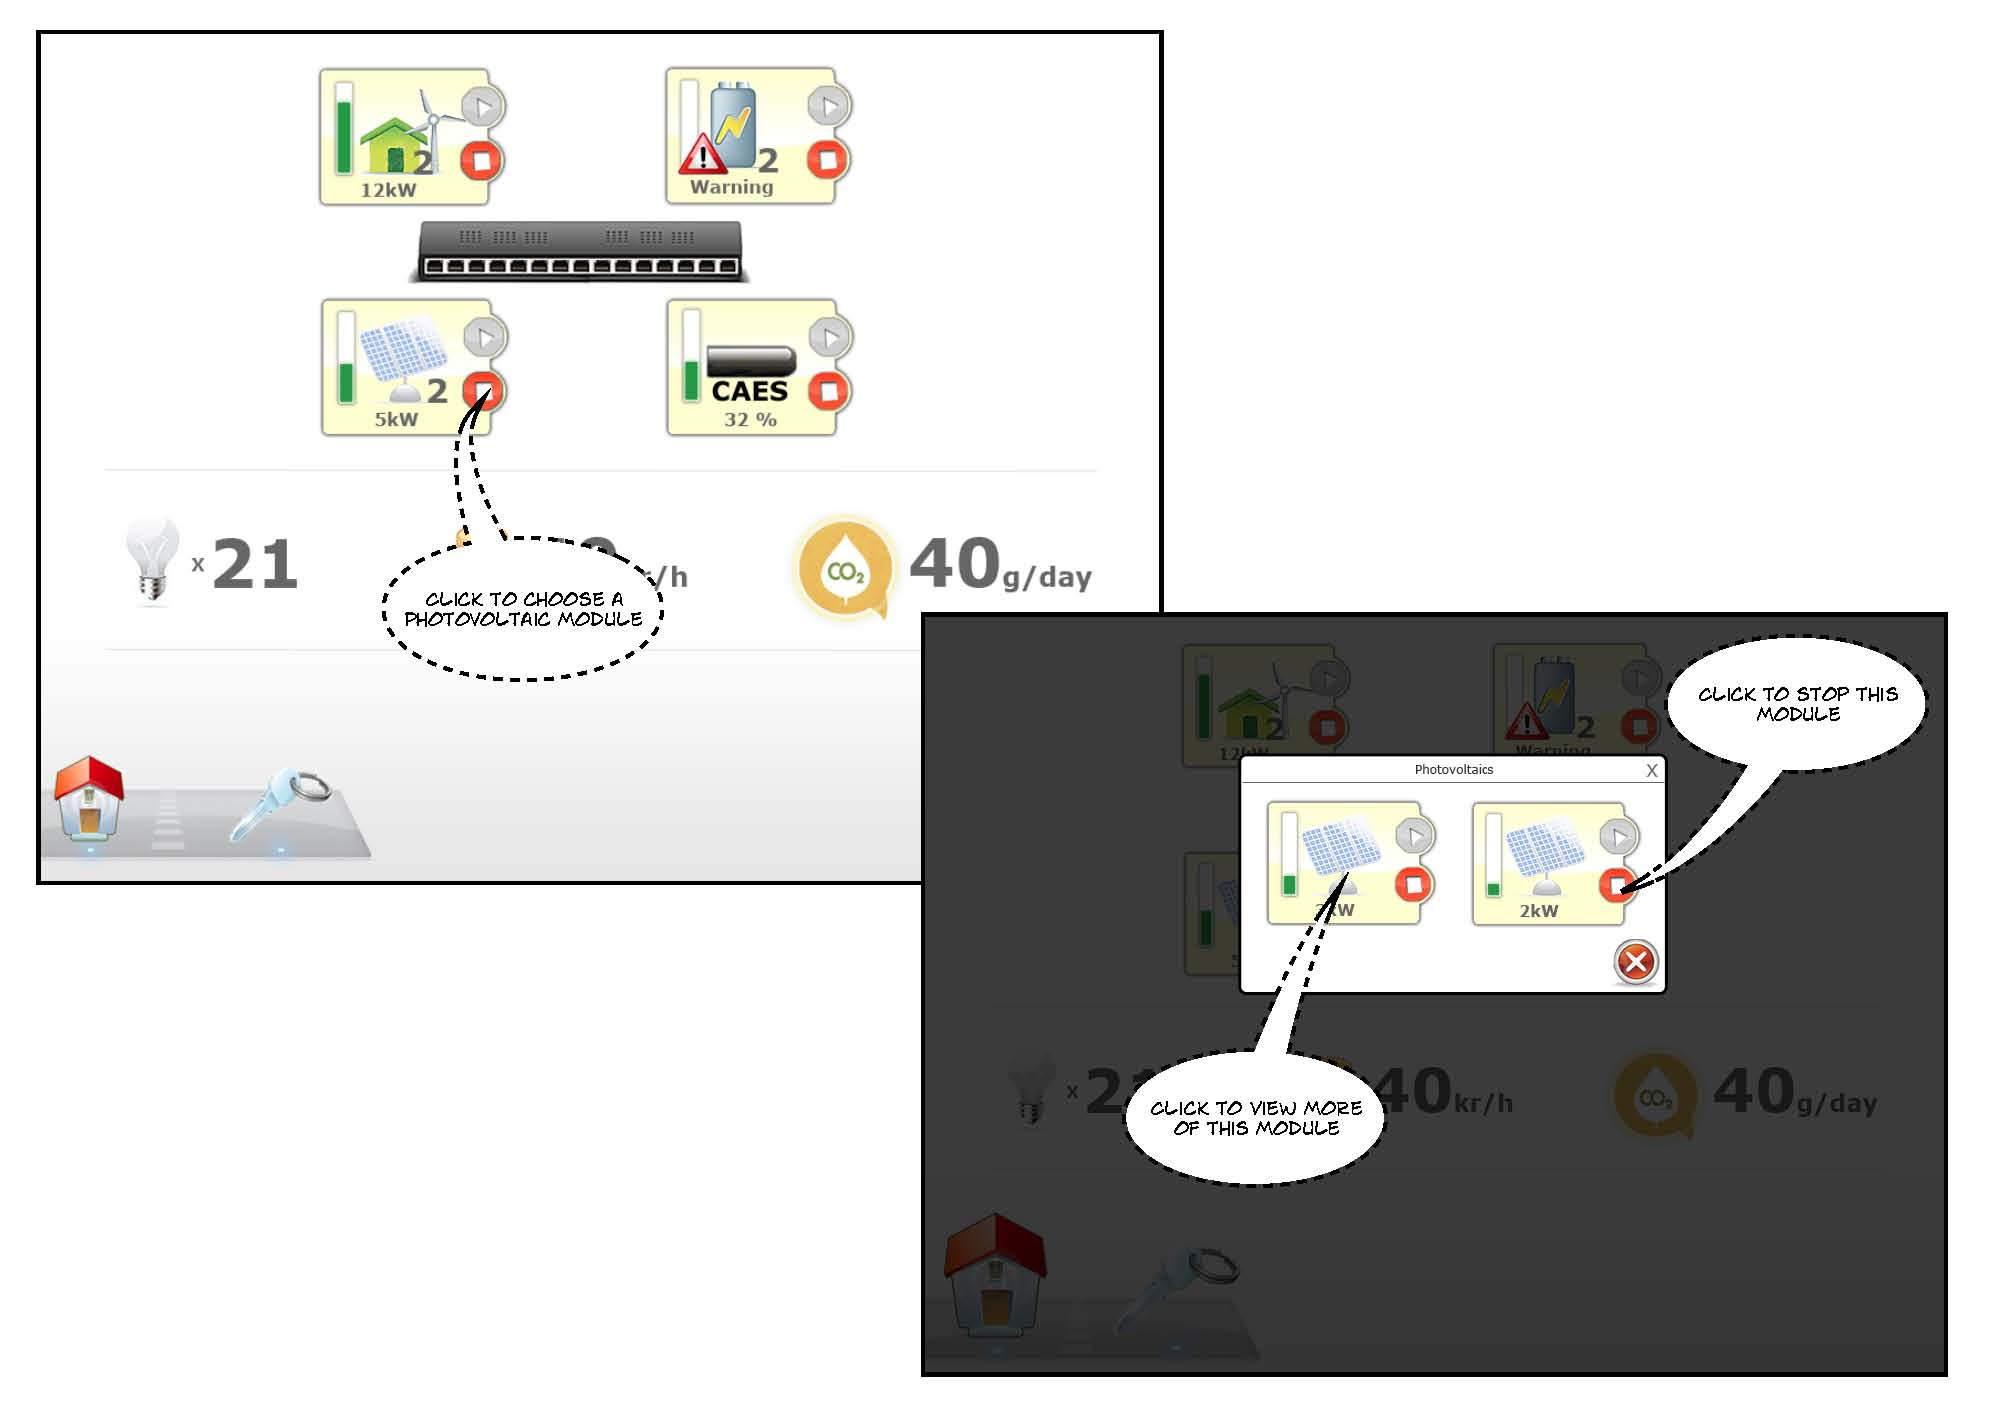
\includegraphics[width=0.68\textwidth]{images/web_interface2.jpg}
				\caption{Web interface; user interaction with the web interface}
		 	\end{centering}
		\end{figure}			
		The energy systems webpage is open for everyone. Everyone can go to the webpage and see the status of the system and all of its sub-devices.
		When the user logs onto the system he gets access to start and stop devices, read the log files, change settings such as, warning mail address,
		password e.g.
	\subsubsection{Function Analysis}
		From an analytic perspective, functions are very useful as they are intended to elaborate the objective of the system. When defining functions the question is, \textit{what is the system supposed to do?} In the usage part, it was concerned \textit{how} the system should be used. This makes the usage and functions closely connected, since it is difficult to talk about how a system is being used without discussing what it should do.\\\\
		When analyzing functions the object is to get a complete list of all the functions the system must implement. The goal is not to describe every single function in detail, quite the contrary the goal is to identify the functions.\\\\
		Functions can be grouped into types. There are four different types of functions:\\\\
		\textit{Update} is a type defining functions which are activated by a problem or application domain event, and which results in a change in the model's state.\\\\
		The type \textit{Signal} defines a function which is triggered by a change in the model's state. Running the function always results in a reaction to its surroundings: that is either the reaction is a display to the actors in the problem domain or else the reacting a direct intervention in the problem domain.\\\\
		When an actor has need for information the function of type \textit{Read} is activated. The function is displaying the relevant data of the model to the actor.\\\\
		Finally, the \textit{Calculating} function is activated when an actor provides information, which should be included in a computation which also involves data from the model. The function returns its computed result to a display.\\\\
		When all functions are found they must be defined by their type and complexity, as below.
		\begin{table}[h!]
			\begin{tabular}{| l | c | c |}
				\hline
	Title																	& Complexity 		& Type			\\ \hline
	A user should be able to connect a new module								& S				& Update 			\\ \hline
	A user should be able to disconnect a module									& S				& Update	 		\\ \hline
	A user should be able to start a module on the system and on the web page			& M				& Update 			\\ \hline
	A user should be able to stop a module on the system and on the web page			& M				& Update 			\\ \hline
	A user should be able to start the system on the system							& S				& Update 			\\ \hline
	A user should be able to see the production of a module on the web page			& M				& Read/Calculating 	\\ \hline
	A user should be able to see the consumption of a module on the web page			& M				& Read/Calculating 	\\ \hline
	A user should be able to see the temperature									& M				& Read 			\\ \hline
	A user should be able to see the humidity										& M				& Read			\\ \hline
	A user should be able to see the log of a module								& M				& Read			\\ \hline
	A user should be able to see the energy level on stoage modules					& M				& Read/Calculating 	\\ \hline
	The system should be able to initialize a module								& C				& Update/Calculating\\ \hline
	The system should be able to shutdown if the temperature gets too low				& M				& Read/Calculating 	\\ \hline
	The system should be able to set a module to standby							& M				& Update 			\\ \hline
	The system should be able to create a log file for new modules					& C				& Update 			\\ \hline
	The system should be able to electrical disconnect modules						& C				& Update 			\\ \hline
	The system should be able to stop modules									& M				& Update	 		\\ \hline
	The system should be able to start modules									& M				& Update		 	\\ \hline
				\end{tabular}
				\caption{S = simple. M = medium. C = complex. VC = very complex}
			\end{table}
	\subsubsection{System Dynamics}
			Diagram of how to put data on the web server.
			\\Small diagram of how to initialize, start, stop, pause submodules.
			\begin{figure}[h!]		%Remember to put the h!, to not fuck the sections.
			\begin{centering}
				 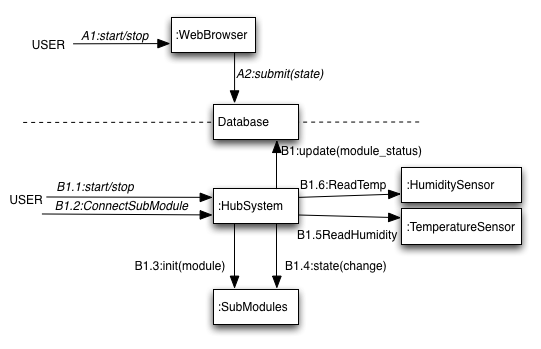
\includegraphics[width=0.7\textwidth]{images/communication_diagram.png}
				\caption{...}
		 	\end{centering}
		\end{figure}		
\subsection{General Architecture Design}
	\subsubsection{Design Criteria}
		Write in what parts should be used (mostly off the shelf things).
				\begin{table}[h!]
					\begin{tabular}{| r | c | c | c | c | c |}
					\hline
					Issue & Critical & Very Important & Important & Less Important & Notes \\ \hline
					Safe					& X & ~ & ~ & ~ & 1 \\ \hline
					Performance 			& ~ & ~ & X & ~ & 2 \\ \hline
					Usage 				& X & ~ & ~ & ~ & 3 \\ \hline
					Reliability 			& X & ~ & ~ & ~ & 4 \\ \hline
					Easy serviceable 		& ~ & X & ~ & ~ & 5 \\ \hline
					Remote maintenance 	& ~ & ~ & X & ~ & 6 \\ \hline
					Cost effective 			& ~ & ~ & ~ & X & 7 \\ \hline
					\end{tabular}
				\end{table}
			Notes:
			\begin{enumerate}
			\item The safety is a very important factor, as the system is meant as a showoff system for high-school students, who should
			be able to be near the system without hurting themselves or the system.
			\item The performance in the system is not critical when considering it from the users perspective. It doesn't matter if it takes a few seconds before the system responds the user.
			But the system should still be able to react fast in order not to harm it self, but also to get a high effectiveness. 
			\item The system should be easy to use. All kinds of people should be able to use the system without any specific training.
			Connecting of new devices and doing administrative jobs on the system a small walk through of the system is required. 
			\item Errors must not occur in the system. The hub is the central nerve in the whole system, therefore if the hub does not run, non of the subsystems does and no energy is routed.
			\item The user of the system should be able to find eventual errors on the system by him self, with help from a good error log created by the system.
			\item The only thing possible to maintain remotely is start and stop of submodules + power down the whole system, which is less important as the system is placed locally.
			\item Only one kind of the system is to be produces, but still the price should be kept at a relatively low level (as we have an undefined maximum price of the system).
			\end{enumerate}
				
	\subsubsection{Subsystem Design}
		\begin{itemize}
			\item Subsystem Architecture Diagram
			\item Detailed Block Diagrams
		\end{itemize}
	\subsubsection{Architecture Dynamics}
		Hubs communication with submodules
		\begin{itemize}
			\item Sequence Diagrams
		\end{itemize}
\subsection{Technical Platform}
	A lot of technical stuffs. 
	\subsubsection{Hardware Specifications}
	\subsubsection{Software Specifications}